%----------------------------------------------------------------------------------------
%    PACKAGES AND THEMES
%----------------------------------------------------------------------------------------

\documentclass[aspectratio=169,xcolor=dvipsnames]{beamer}
\usetheme{SimplePlus}

\usepackage{tikz}
\usepackage{hyperref}
\usepackage{graphicx} % Allows including images
\usepackage{booktabs} % Allows the use of \toprule, \midrule and \bottomrule in tables
\usepackage{wrapfig}
\usepackage{listings}

%----------------------------------------------------------------------------------------
%    TITLE PAGE
%----------------------------------------------------------------------------------------

\title{Introduction to R Language}
\subtitle{HI 743}

\author{}

\institute
{
    Department of Health Informatics and Administration \\
    Zilber College of Public Health \\
    University of Wisconsin - Milwaukee% Your institution for the title page
}
\date{February 6, 2025} % Date, can be changed to a custom date

%----------------------------------------------------------------------------------------
%    PRESENTATION SLIDES
%----------------------------------------------------------------------------------------

\begin{document}
\begin{frame}
    % Print the title page as the first slide
    \titlepage
\end{frame}
%----------------------------------------------------------------------------------------

\begin{frame}{R \& RStudio}
R was created during the 1990's as a derivative of the S programming language. Recently it has risen to popularity for reasons including:
\vspace{0.5cm}
\begin{itemize}
\item R is open source and freely available.
\item R is available for Windows, Mac, and Linux.
\item R has an extensive set of tools for statistical analysis.
\item R has an extensive, flexible graphical facility capable of producing publication quality figures.
\item R has an expanding set of freely available 'packages' to extend R's capabilities.
\item R has an extensive support network with numerous online resources.

\end{itemize}
\end{frame}

%----------------------------------------------------------------------------------------

\begin{frame}{Comprehensive R Archive Network (CRAN)}

The “Comprehensive R Archive Network” (CRAN) is a collection of sites which carry identical material, consisting of the R distribution(s), the contributed extensions, documentation for R, and binaries.

\begin{center}
https://CRAN.R-project.org/
\end{center}

From CRAN, you can obtain the latest official release of R, daily snapshots of R (copies of the current source trees), as gzipped and bzipped tar files, a wealth of additional contributed code, as well as prebuilt binaries for various operating systems (Linux, Mac OS Classic, macOS, and MS Windows). CRAN also provides access to documentation on R, existing mailing lists and the R Bug Tracking system.

\end{frame}


%----------------------------------------------------------------------------------------
\begin{frame}{Why use R? Open Source.}
R is released under the GNU General Public License (GPL), version 2 or version 3. The GPL is a free software license that guarantees users the freedom to run, study, modify, and distribute software. It explicitly encourages using this software in all contexts with freedom from proprietary restrictions.

\vspace{.5cm}

It is the opinion of the R Core Team that one can use R for commercial purposes (e.g., in business or in consulting). The GPL, like all Open Source licenses, permits all and any use of the package. Most add-on packages, including all recommended ones, also explicitly allow commercial use in this way. 

\end{frame}



%----------------------------------------------------------------------------------------
\begin{frame}{Why use R? Packages.}

R packages are extensions to the R statistical programming language. R packages contain code, data, and documentation in a standardized collection format that can be installed by users of R, typically via a centralized software repository. The two most popular software repositories are:
\vspace{0.25cm}
\begin{itemize}
	\item \textbf{CRAN}: is R's central software repository. As of November 2020, more than 16,000 packages are available. The master site is located at the Vienna University of Economics and Business and is mirrored on servers around the world.
	\item \textbf{Bioconductor}: project provides R packages for the analysis of genomic data. This includes object-oriented data-handling and analysis tools for data from Affymetrix, cDNA microarray, and next-generation high-throughput sequencing methods.
\end{itemize}
\end{frame}


%----------------------------------------------------------------------------------------
\begin{frame}{RStudio Orientation}
RStudio is an \textbf{Integrated Development Environment} (IDE). RStudio can be thought of as an add-on to R which provides a more user-friendly interface, incorporating the R Console, a script editor and other useful functionality (like R markdown and GitHub integration).

\vspace{0.5cm}

RStudio includes a console, syntax-highlighting editor that supports direct code execution, and a variety of robust tools for plotting, viewing history, debugging and managing your workspace.
\end{frame}

%----------------------------------------------------------------------------------------
\begin{frame}{RStudio Orientation}
When you open RStudio for the first time, you will see the following layout.
\begin{center}
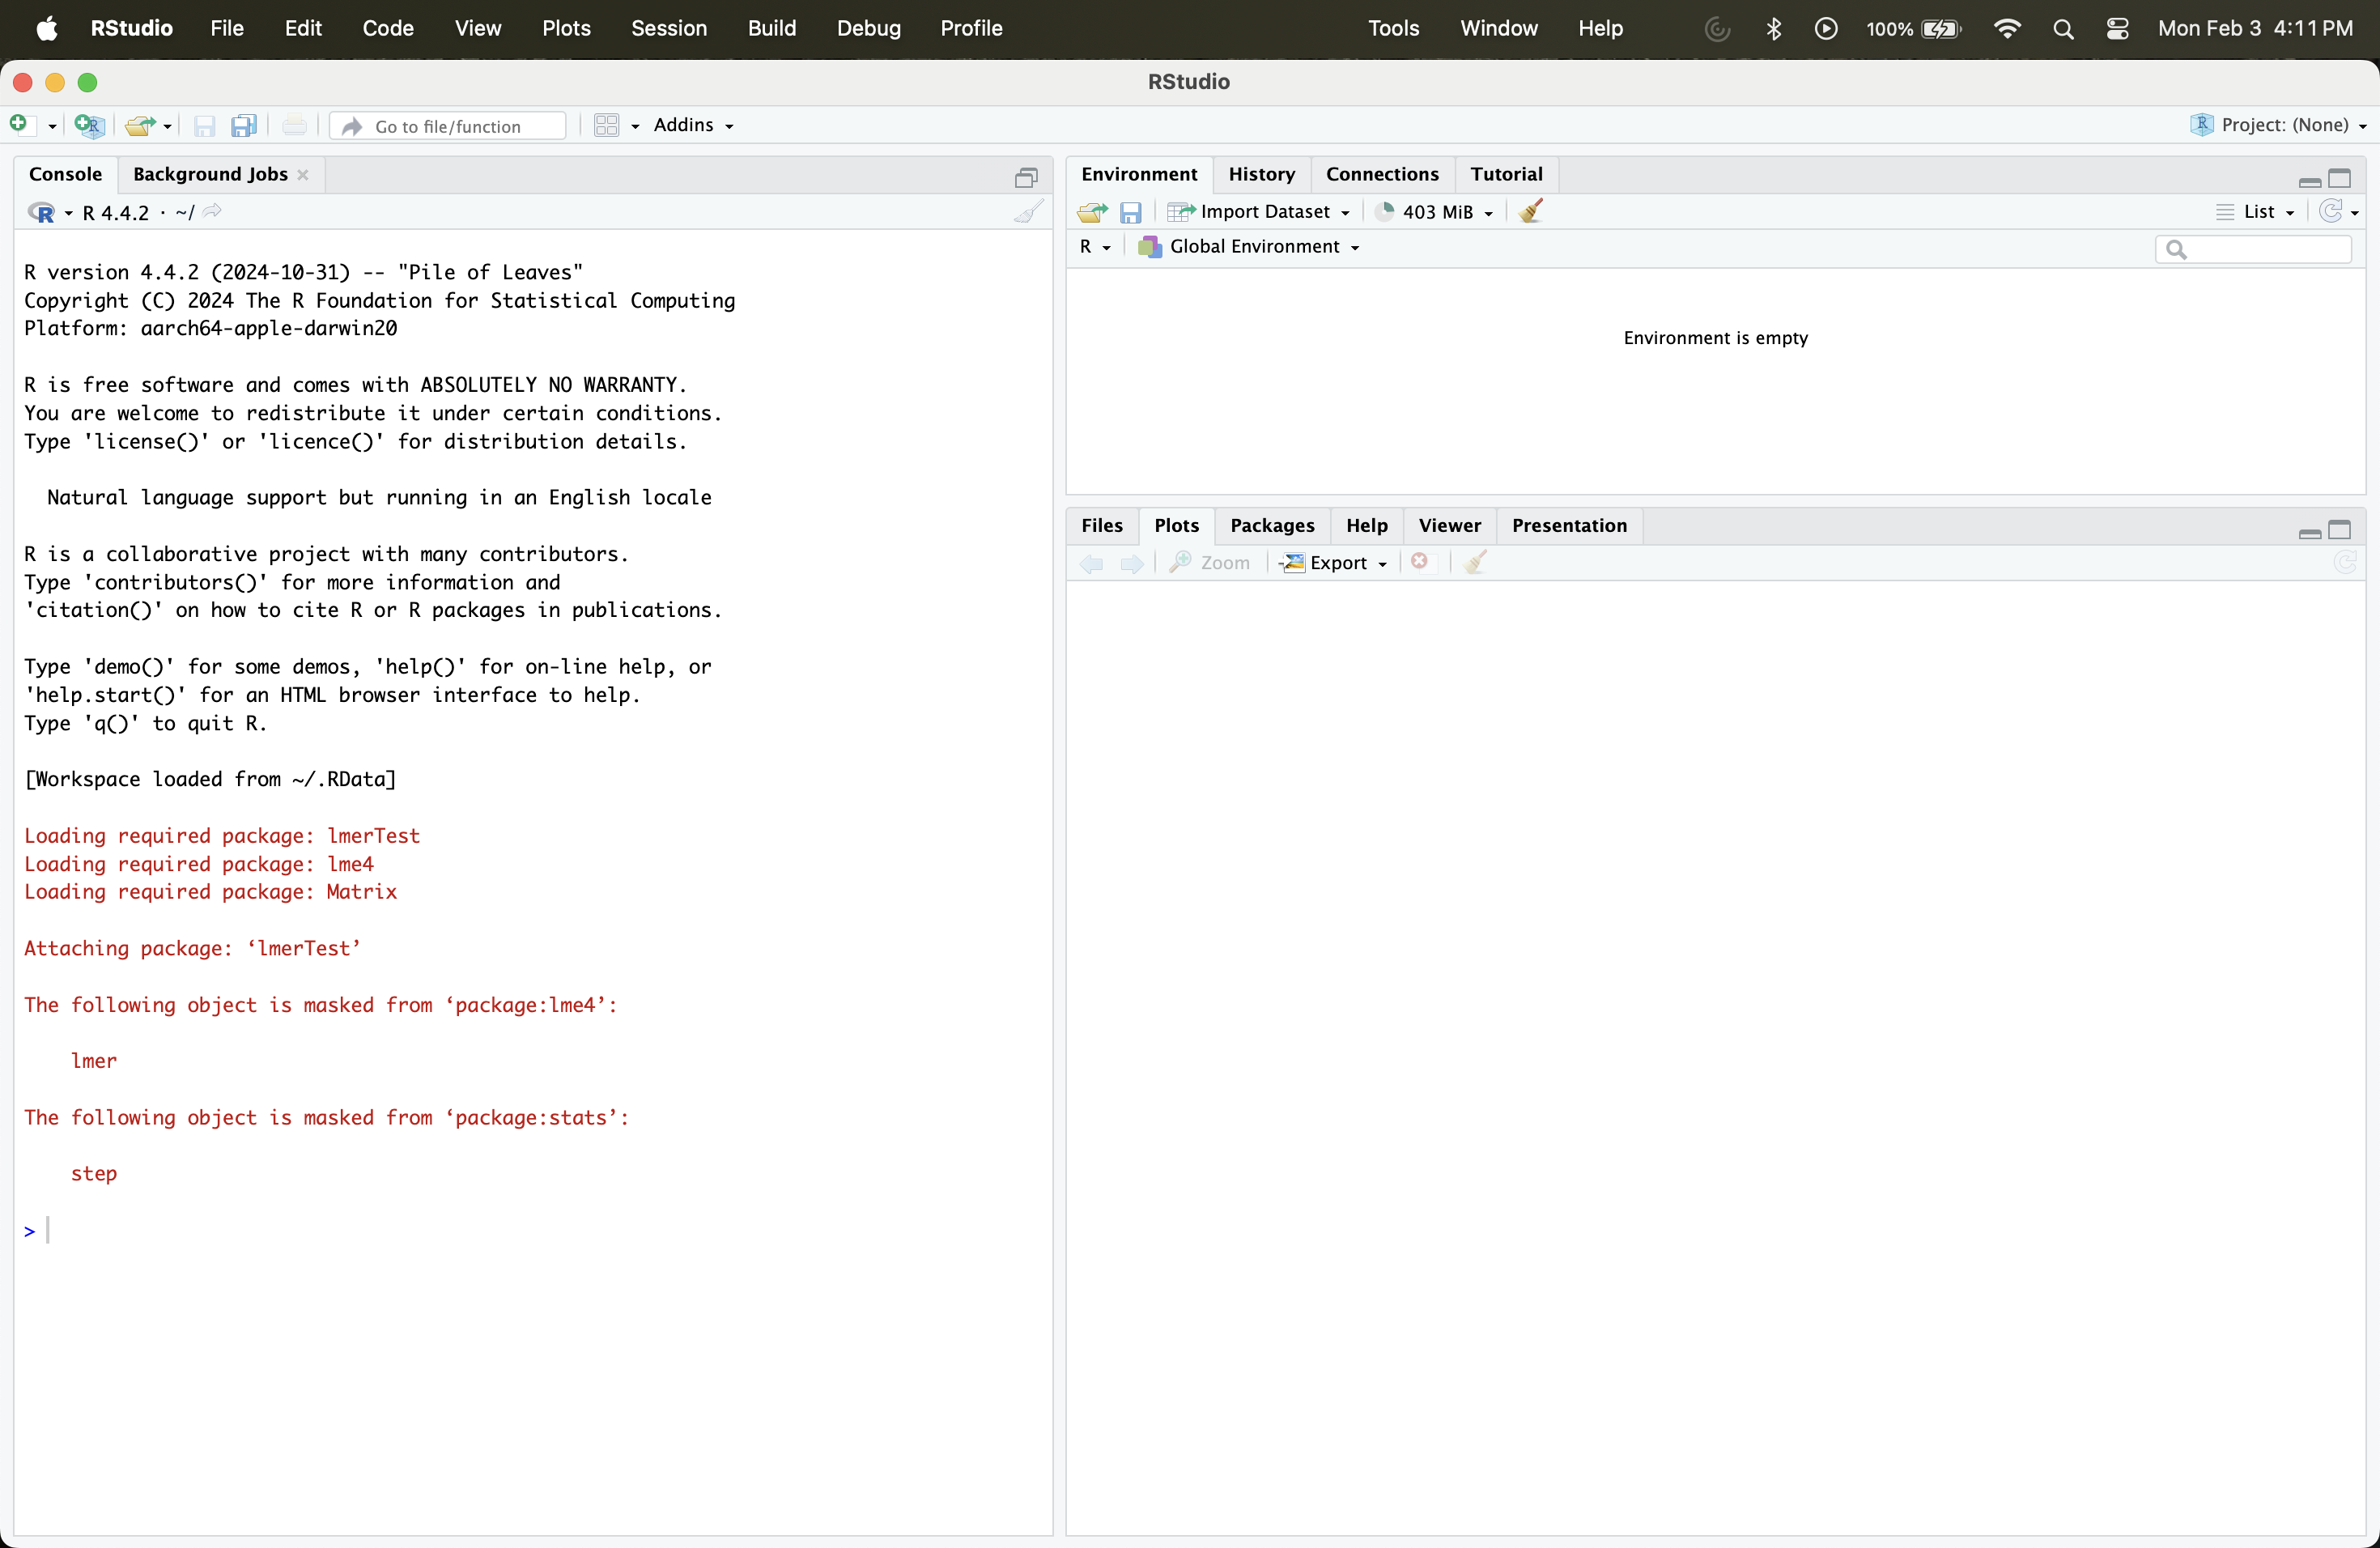
\includegraphics[scale=0.2]{images/Rstudio.png}
\end{center}

\end{frame}

%----------------------------------------------------------------------------------------
\begin{frame}{RStudio Orientation: Console}
The Console is the workhorse of R. This is where R evaluates all the code you write. You can type R code directly into the Console at the command line prompt, $>$. For example, if you type 2 + 2 into the Console you should obtain the answer 4.
\begin{center}
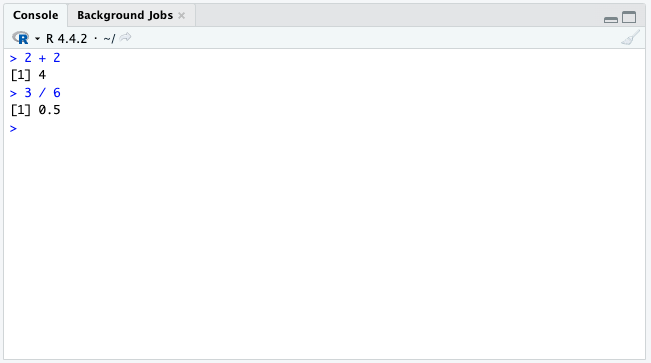
\includegraphics[scale=0.4]{images/console.png}
\end{center}
\end{frame}

%----------------------------------------------------------------------------------------
\begin{frame}{RStudio Orientation: Console}
\begin{columns}
        \begin{column}{0.5\textwidth}
            Instead of typing R code directly into the Console a better approach is to create an R script.
             An R script is just a plain text file with a .R file extension which contains your lines of R code. 
             These lines of code are then sourced into the R Console line by line. \\
             \vspace{0.5cm}
             The [$\rightarrow$Run] button in the top-right will run the entire script in the source pane. Otherwise, 'Command+Enter' (Ctrl+Enter on Windows) will run the current line, or the highlighted block of text.
        \end{column}

        \begin{column}{0.5\textwidth}
            \centering
            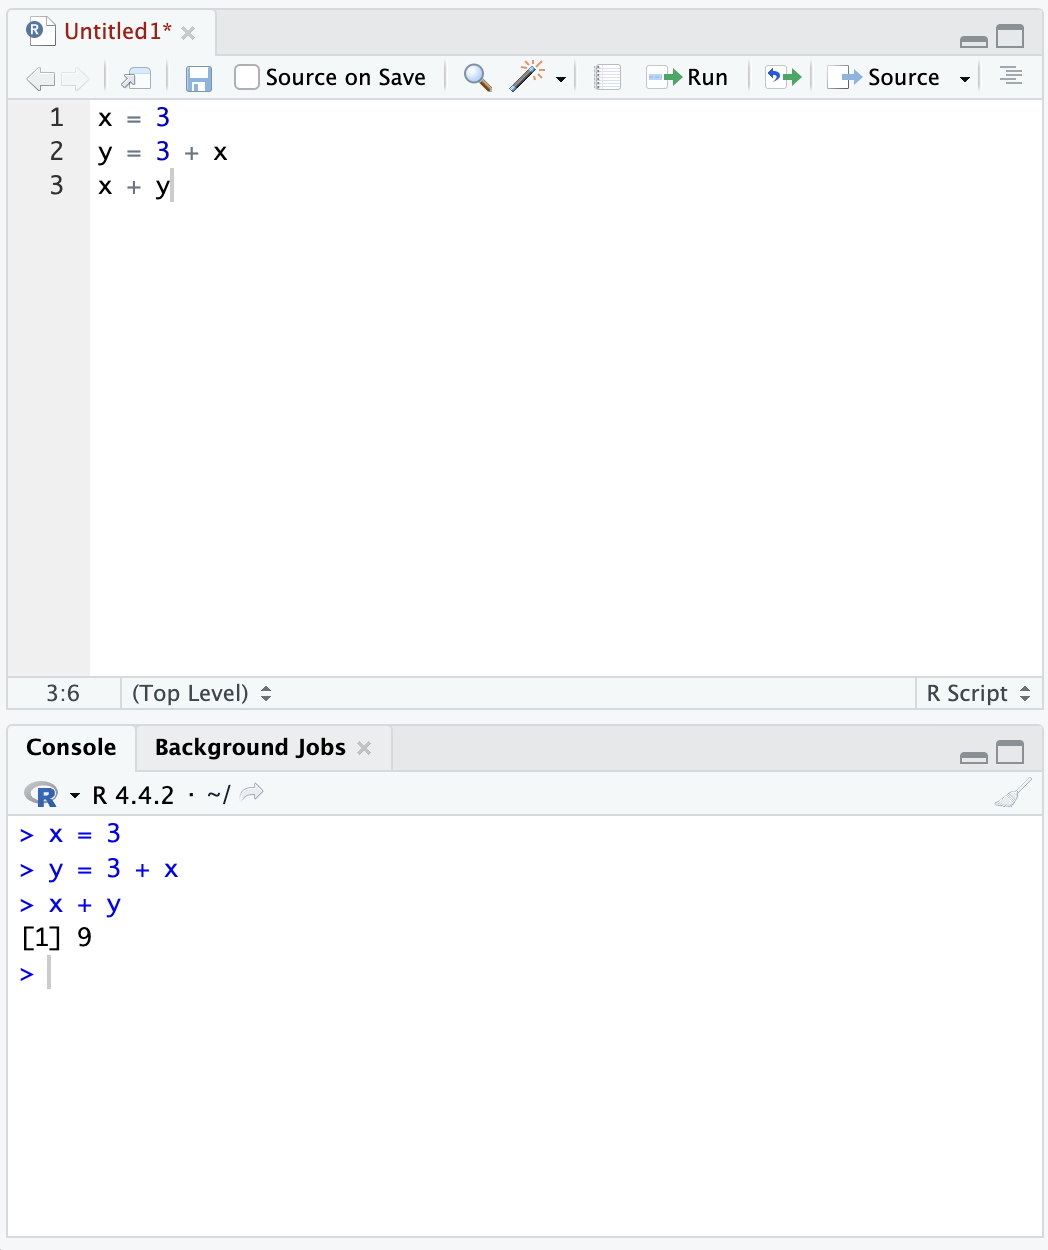
\includegraphics[scale=0.32]{images/source.png}
        \end{column}
    \end{columns}
\end{frame}
%----------------------------------------------------------------------------------------

\begin{frame}{RStudio Orientation: Top-Right Panel}

\begin{columns}
        \begin{column}{0.5\textwidth}
	\begin{itemize}
	\item The \textbf{Environment} tab displays all the objects you have created in the current (global) environment. 
	\item The \textbf{History} tab contains a list of all the commands you have entered into the R Console.
	\item The \textbf{Connections} tab allows you to connect to various data sources such as external databases.
	\end{itemize}
        \end{column}

        \begin{column}{0.5\textwidth}
            \centering
            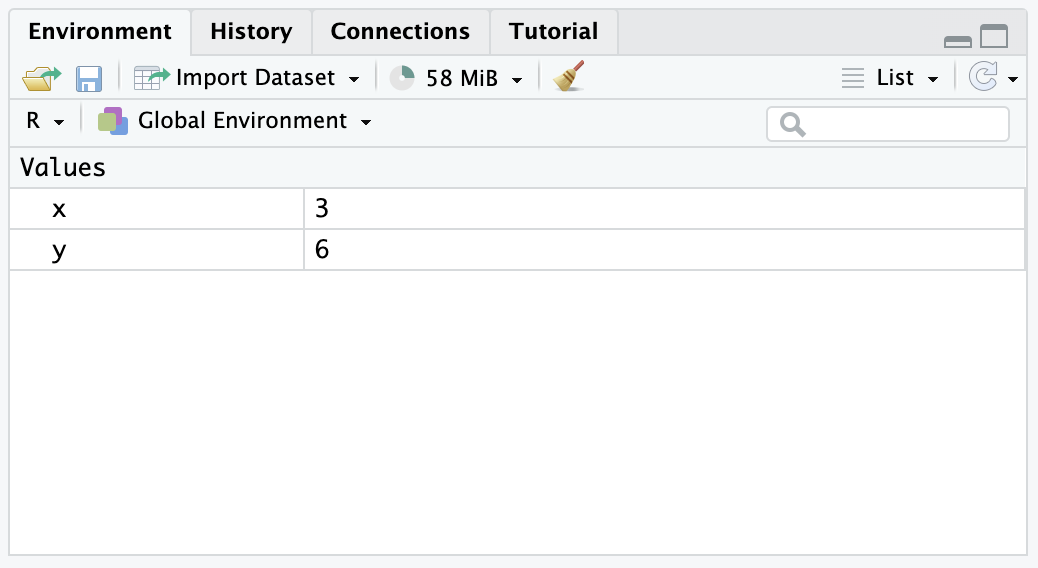
\includegraphics[scale=0.32]{images/env.png}
        \end{column}
    \end{columns}
\end{frame}

%----------------------------------------------------------------------------------------
\begin{frame}{RStudio Orientation: Bottom-Right Panel}
\begin{columns}
        \begin{column}{0.5\textwidth}
	\begin{itemize}
	\item  The \textbf{Files} tab lists all external files and directories in the current working directory on your computer.
	\item The \textbf{Plots} tab is where all the plots you create in R are displayed (unless you tell R otherwise).
	\item The \textbf{Packages} tab lists all of the packages that you have installed on your computer.
	\item The \textbf{Help} tab displays the R help documentation for any function.
	\item The \textbf{Viewer} tab displays local web content such as web graphics generated by some packages.
	\end{itemize}
        \end{column}

        \begin{column}{0.5\textwidth}
            \centering
            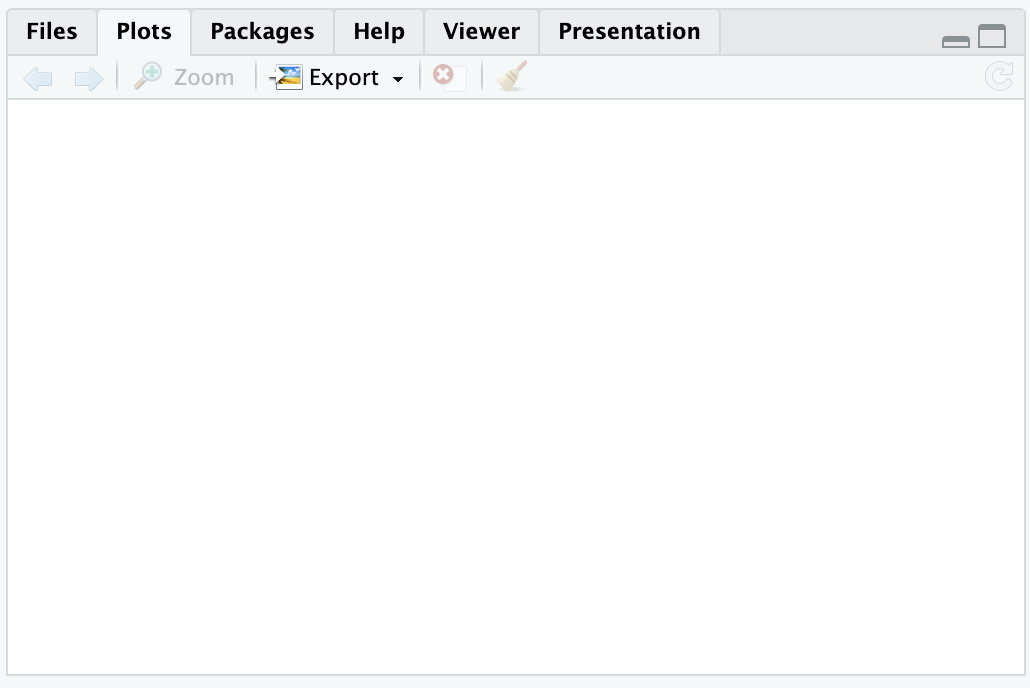
\includegraphics[scale=0.32]{images/files.png}
        \end{column}
    \end{columns}
\end{frame}

%----------------------------------------------------------------------------------------
\begin{frame}{Packages: CRAN}
To install a package from CRAN you can use:

\begin{block}{Install Packages Function}
	\texttt{install.packages()}
\end{block}
 
 For example if you want to install the remotes package enter the following code into the Console window of RStudio \\
 \begin{center}
 \texttt{install.packages("ISLR", dependencies = TRUE)}
 \end{center}
You can also use the following function to update existing packages.
\begin{block}{Update Packages Function}
	\texttt{update.packages()}
\end{block}

\end{frame}


%----------------------------------------------------------------------------------------
\begin{frame}{Packages: Bioconductor}
To install packages from Bioconductor, you first need to install the \texttt{BiocManager} package. Once the BiocManager package has been installed you can either install all of the ‘core’ Bioconductor packages with:
\begin{block}{Bioconductor Packages}
	\texttt{BiocManager::install()}
\end{block}
\texttt{BiocManager::install(c("GenomicRanges", "edgeR"))} \\
\vspace{0.75cm}
\textbf{Note:} The `::` notation specifies which package specifically to call a function from.

\end{frame}

%----------------------------------------------------------------------------------------
\begin{frame}{Packages: GitHub}
The most efficient method for installed directly from GitHub is to use the \texttt{install\_github()} function from the \texttt{remotes} package.\\
\begin{block}{GitHub Packages}
	\texttt{remotes::install\_github('tidyverse/dplyr')}
    \end{block}

\vspace{0.25cm}
Typically, one would install from GitHub if they're looking to use a development version of an R Package. It's important to note that installing from GitHub could add security risks if the repository is not properly vetted.

\end{frame}

%----------------------------------------------------------------------------------------
\begin{frame}{Working Directories}
The working directory is the default location where R will look for files you want to load and where it will put any files you save. You can check the file path of your working directory by looking at bar at the top of the Console pane. You can also use the \texttt{getwd()} function in the Console which returns the file path of the current working directory.
\begin{center}
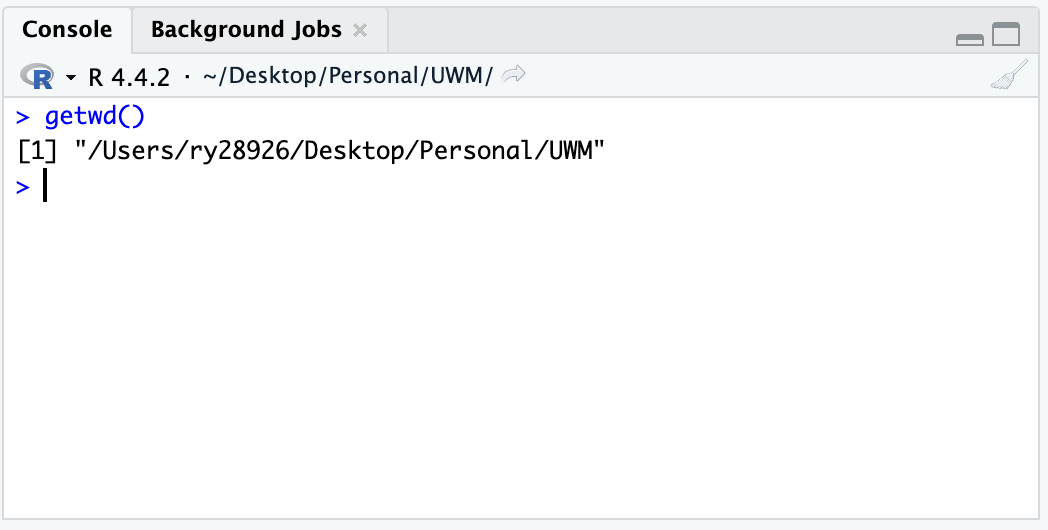
\includegraphics[scale=0.5]{images/getwd.png}
\end{center}
\end{frame}

%----------------------------------------------------------------------------------------
\begin{frame}{Working Directories}
The \texttt{setwd()} function will allow you to change your working directory. This can help reduce the amount of typing needed to locate files that exist together. It will also be where files save-to by default. 


\begin{center}
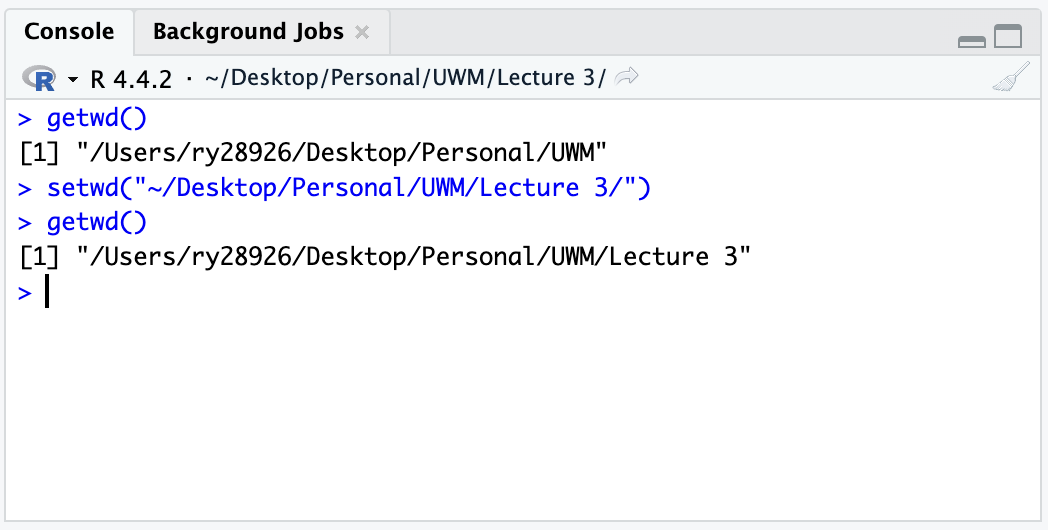
\includegraphics[scale=0.5]{images/setwd.png}
\end{center}
\end{frame}
%----------------------------------------------------------------------------------------
\begin{frame}{Recommended Project Directory Structure}

\begin{columns}
        \begin{column}{0.5\textwidth}
	It’s good practice to structure your working directory in a consistent and logical way to help both you and your collaborators. Shown is a recommended directory structure.
        \end{column}

        \begin{column}{0.5\textwidth}
            \centering
            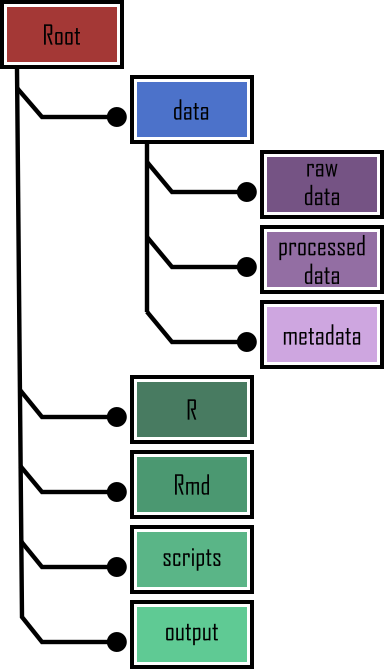
\includegraphics[scale=0.33]{images/dir.png}
        \end{column}
    \end{columns}
\end{frame}

%----------------------------------------------------------------------------------------
\begin{frame}{Project Documentation}
It's important include in your R script all the information required to make your work reproducible (author names, dates, sampling design etc). Comments can be made with the \textbf{\#} symbol. \\

\begin{center}
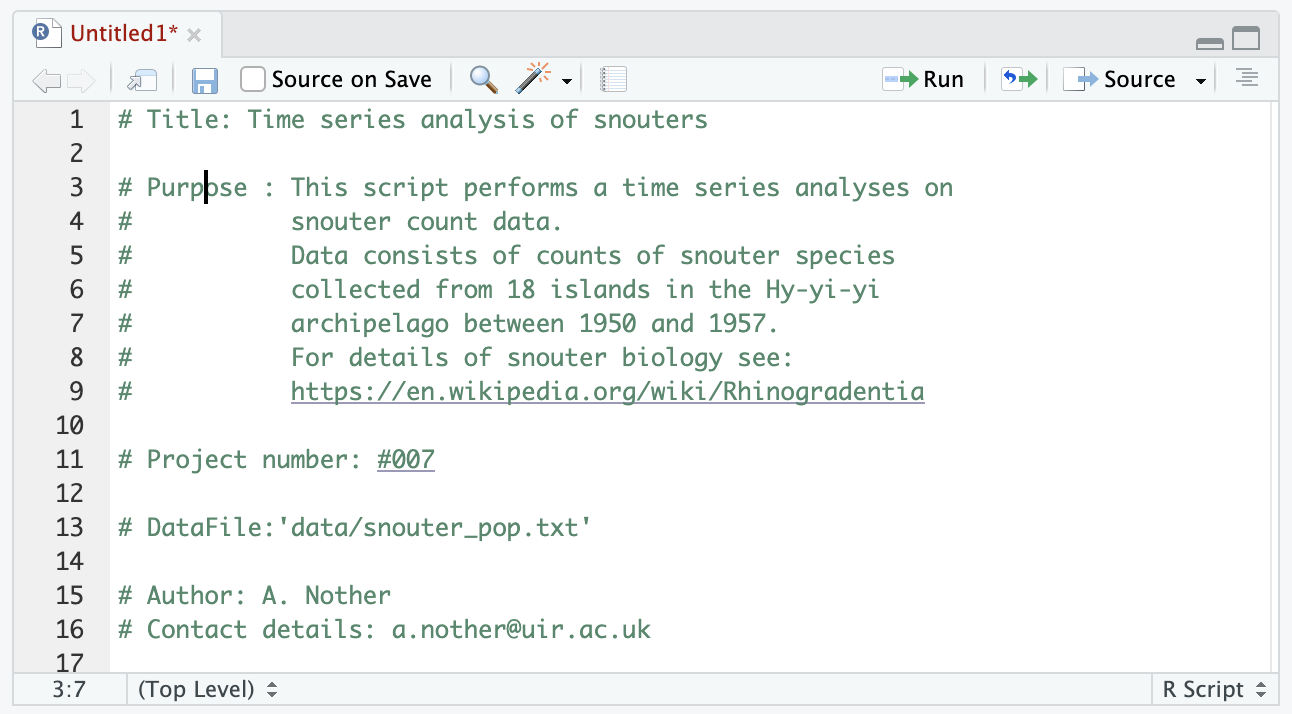
\includegraphics[scale=0.4]{images/documentation}
\end{center}
\end{frame}

%----------------------------------------------------------------------------------------
\begin{frame}[fragile]{Objects in R}
A main concept in R is that everything is an \textbf{object}. \\
\vspace{0.5cm}
These objects can be almost anything, from a single number or character string (like a word) to highly complex structures like the output of a plot, a summary of your statistical analysis or a set of R commands that perform a specific task. \\

\begin{center}
\begin{lstlisting}[language=R]
    > my_obj = 48
    > my_obj
    ## [1] 48
    \end{lstlisting}
\end{center}

\end{frame}


%----------------------------------------------------------------------------------------
\begin{frame}[fragile]{Objects in R}
Now that we’ve created this object, R knows all about it and will keep track of it during this current R session. All of the objects you create will be stored in the current workspace and you can view all the objects in your workspace in RStudio by clicking on the ‘Environment’ tab in the top right hand pane.

\begin{center}
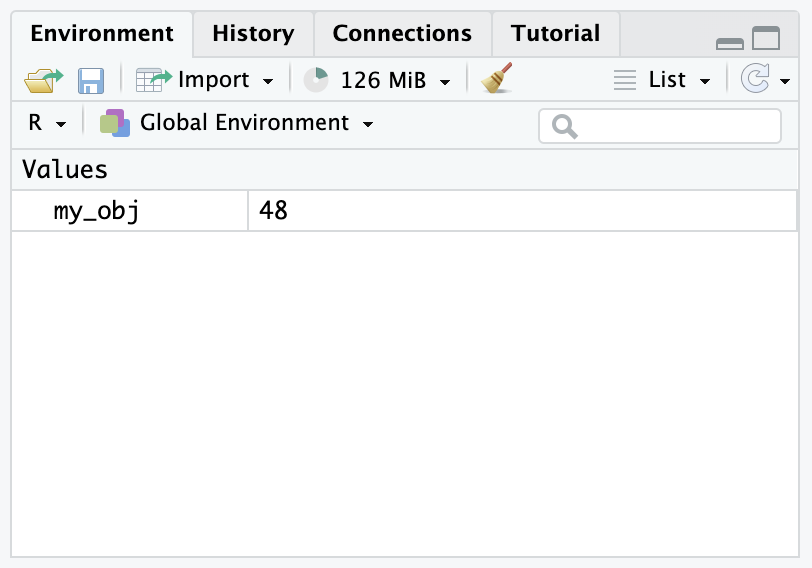
\includegraphics[scale=0.4]{images/env_obj.png}
\end{center}
\end{frame}

%----------------------------------------------------------------------------------------
\begin{frame}[fragile]{Objects in R}
If you click on the down arrow on the ‘List’ icon in the same pane and change to ‘Grid’ view RStudio will show you a summary of the objects including the type (numeric - it’s a number), the length (only one value in this object), its ‘physical’ size and its value (48 in this case).
\begin{center}
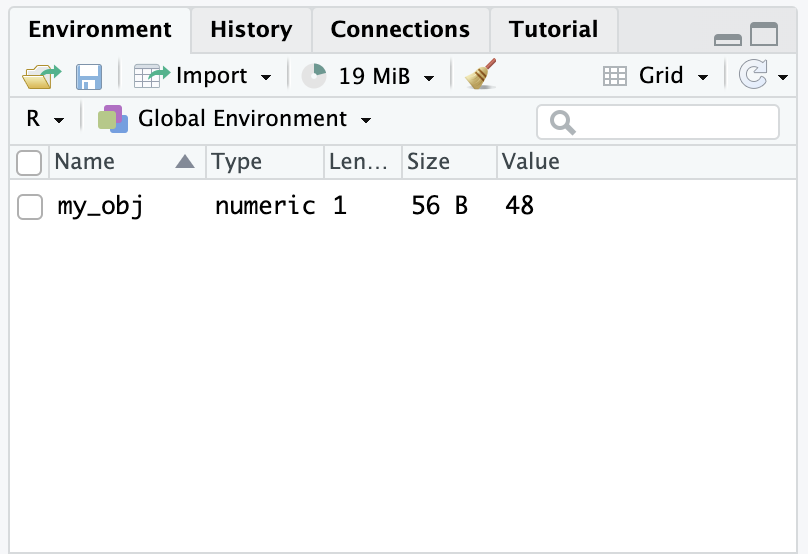
\includegraphics[scale=0.4]{images/env_grid.png}
\end{center}
\end{frame}

%----------------------------------------------------------------------------------------
\begin{frame}[fragile]{Objects in R}
There are many \textit{types} of objects that we can assign values to. For instance, we can create a \textit{character} type variable. \\

\begin{center}
\begin{lstlisting}[language=R]
    > my_obj2 = "R is cool"
    > my_obj2
    ## [1] "R is cool"
    \end{lstlisting}
\end{center}
\begin{center}
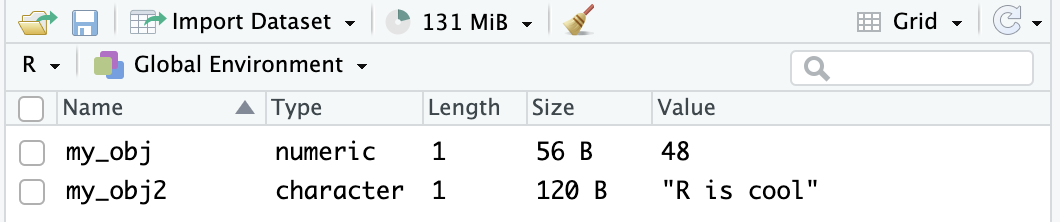
\includegraphics[scale=0.4]{images/env_cool.png}
\end{center}
Notice that we have enclosed the string in quotes. If you forget to use the quotes you will receive an error message. \\ 

\end{frame}

%----------------------------------------------------------------------------------------


\begin{frame}{Bibliography}
\begin{enumerate}
	\item https://cran.r-project.org/
	\item https://intro2r.com/
\end{enumerate}
\end{frame}

\end{document}